\documentclass[pdftex,14pt,a4paper]{extreport}
\usepackage[utf8]{inputenc} %koi8-r + cyrillic encoding
\usepackage[bulgarian]{babel}

\usepackage[pdftex]{graphicx}
\usepackage{hyperref}
\usepackage{listings}
\lstset{
  frame=single,
  numbers=left
}
\usepackage{float}
\usepackage{./titlesec/titlesec}
\titleformat{\chapter}[display]
{\normalfont\huge\bfseries}{\chaptertitlename\ \thechapter}{20pt}{\Huge}

% this alters "before" spacing (the second length argument) to 0
\titlespacing*{\chapter}{0pt}{0pt}{40pt}
\hypersetup{
 	colorlinks = true,
  linkcolor = black
}

\newcommand{\HRule}{\rule{\linewidth}{0.5mm}}

\begin{document}
\setcounter{secnumdepth}{3}
\setcounter{tocdepth}{3}
\begin{titlepage}
	\begin{center}
		{\Huge ТЕХНОЛОГИЧНО УЧИЛИЩЕ ЕЛЕКТРОННИ СИСТЕМИ\\[0.5cm]} {\Large към ТЕХНИЧЕСКИ УНИВЕРСИТЕТ - СОФИЯ\\[3cm]}
		{\Huge ДИПЛОМНА РАБОТА\\[3cm]}
		Тема: ''Мултитенант'' система за управление на интернет сайтове\\[3cm]
		\begin{minipage}{0.4\textwidth}
			\begin{flushleft} \large
				\emph{Дипломант:}\\
				Михаил \textsc{Здравков}
			\end{flushleft}
		\end{minipage}
		\begin{minipage}{0.4\textwidth}
			\begin{flushright} \large
				\emph{Научен ръководител:} \\
				Инж.~Кирил \textsc{Митов}
			\end{flushright}
		\end{minipage}

		\vfill

		% Bottom of the page
		{\large София 2014}

	\end{center}
\end{titlepage}
\tableofcontents
\listoftables
\listoffigures
\pagebreak
\phantomsection
\chapter*{Увод}
\addcontentsline{toc}{part}{Увод}
Some увод
\chapter {Преглед на подобни продукти. Обзор на софтуерни технологии}
\section {Преглед на подобни продукти}
Някои приложения и решения доближаващи се по функционалност до разработваната дипломна работа (макар и само в някои аспекти):
\subsection {Heroku}
Heroku\footnote{Източник на информацията за Heroku са \url{https://www.heroku.com} и \\\url{https://devcenter.heroku.com/articles/quickstart}} е платформа за хостване на Интернет приложения на облачно базиран сървър\footnote{облачно базиран сървър е мрежа от компютри, която предоставя изчислителни ресурси на клиента.}, която може да бъде използвана за приложения, написани на редица програмни езици (някои от които са Ruby, Clojure, Python, Java и Scala). Целта на Heroku е да позволи на клиентите си да се фокусират над правенето на приложения, а не на инфраструктура. Управлението на приложенията се извършва чрез командния ред, а изпращането на програмния код чрез Git (популярна система за управление на версиите). Heroku позволява лесен разтеж на приложението - това става чрез система, която дава възможност да скалирате ресурсите, до които приложението ви има достъп. Heroku са въвели модел на стандартна, изчислителна, работна единица, която те наричат Dyno. Всяка една такава единица е лек (взима малко ресурси), изолиран контейнер, в който работи клиентското приложение. Всяко Dyno се равнянва на 512 мегабайта оперативна памет и приоритет 1 в поделянето на процесорно време. С други думи, ако приложението на клиента изведнъж получи извънредно много заявки от клиенти, потребителя на Heroku може да увеличи броя Dyno-та, които използва и да получи повече ресурси от сървърите на Heroku, а когато количеството посещения на приложението му се нормализира, да намали броя Dyno-та, така че да не заплаща ресурси, които не използва.\\\\
Съществуват някои съществени разлики в поставените цели при Heroku и при разработваната дипломна работа, които водят до множество разлики при реализацията и при начина на употреба на двете системи. Heroku е създадена за да работи с различни приложения. Иначе казано, всеки клиент на системата може да качи своето приложение и то няма нищо общо с всички останали. Дипломната работа е създадена да работи с едно единствено приложение, което случи като шаблон за създаването на останалите. Разликата е, че Heroku е създадена за да помогне на програмиста да инсталира някъде своето приложение, докато дипломната работа дава възможност на всякакви потребители да получат свое копие на шаблонното приложение.\\\\
На фигура 1.1 е показано таблото за управление на уеб приложение инсталирано на Heroku.
\begin{figure}[H]
  \centering
  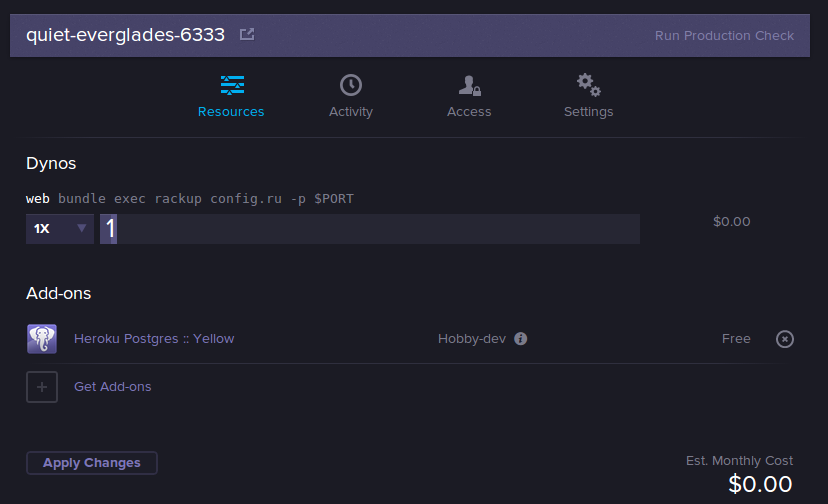
\includegraphics [scale=0.5]{./heroku_dashboard}
  \caption {Табло за управление на уеб приложение на Heroku}
\end{figure}
\section {Обзор на софтуерни технологии}
\subsection {HTTP сървъри}
В тази секция ще разгледаме някои от популярните възможни приложения за предоставяне на съдържание в Интернет.
\subsubsection {Apache}
Apache\footnote{Източници на информацията за Apache HTTP Server са \url{http://news.netcraft.com/archives/category/web-server-survey} и \url{http://www.ntchosting.com/apache-web-server.html}} HTTP Server или само Apache е уеб сървър с отворен код, който има ключова роля за първоначалното разрастване на WWW (World Wide Web). Чрез него работят над 70\% от сайтовете. Счита се от много специалисти за платформа, според която се разработват и оценяват другите уеб сървъри.
Приложението стартира на много операционни системи, включително Unix, GNU, FreeBSD, Linux, Solaris, Mac OS X, Microsoft Windows, OS/2, Novell NetWare и други платформи.
Apache се разработва от отворено общество от разработчици - Apache Software Foundation. Сървърът има възможности за промяна на съобщенията за грешки, удостоверяване на потребителите, договаряне на съдържанието (изключително полезно при многоезични сайтове), proxy модул, както и поддръжка на CGI и SSI. Има множество модули за Apache, които позволяват работа на разнообразни скриптове и осигуряване на динамично съдържание, криптиране, ограничаване и други.
\subsubsection {nginx}
nginx\footnote{Източници на информацията за nginx са \url{http://nginx.com/} и \url{https://nginx.org}} е високопроизводителен уеб сървър и прокси под BSD лиценз. Подобно на други приложения от този вид, архитектурата на nginx е модулна - при компилиране на софтуера се определя кои модули да бъдат вградени в него. Съществуват и над 20 потребителски модула.
nginx може да се използва като обратен прокси сървър, който прехвърля всички или само определени заявки към други физически сървъри. Крайните сървъри могат се избират от nginx на ротационен принцип, но решенията кой от тях да се използва могат да се взимат и чрез по-сложни алгоритми, благодарение на допълнителни модули. Често срещана употреба на приложението е за обработване на заявки за статично съдържание и прехвърляне на по-сложните заявки за динамично съдържание към по-сложен уеб сървър, например Apache. Въпреки това, nginx има пълна FastCGI поддръжка и може да изпълнява скриптове на всеки език за програмиране, който поддържа този стандарт. Софтуерът може да се използва и като SMTP, POP3 и IMAP прокси сървър.
При определени ситуации, особено при обслужване на заявки за статично съдържание, nginx е по-бърз и заема по-малко ресурси от конкурентния софтуер - Apache и lighttpd.
\subsection {Технологии за създавне на Интернет приложения}
\subsubsection {MVC}
Модел-Изглед-Контролер (Model-View-Controller или MVC) е архитектурен шаблон за дизайн (design pattern) в програмирането, основан на разделянето на бизнес логиката от графичния интерфейс и данните в дадено приложение.
\begin{itemize}
  \item Model е частта от програмния код, която представя данните от реалния свят, върху които работим и които сме моделирали. Често моделът служи за свързване с база данни. Основната бизнес логика свързана с обработката на данните се извършва в моделите.
  \item View е частта от програмния код, която описва как ще изглежда уеб страницата, която потребителя ще види. В нея се избягва да има програмна логика и данните, които тя показва се взимат от моделите посредством контролерите.
  \item Controller е частта от програмния код, която служи за връзка между моделите и изгледите. Тя се занимава с това да взима нужната информация от модела и да я предоставя на изгледа. В нея се извършват също дейности като уторизация на потребителите, обработка на параметри от HTTP заявки и пренасочване към други страници.
\end{itemize}
MVC носи значителни предимства при разработването на уеб приложения. Модулярността позволява да направите различен интерфейс за същите модели, като промените единствено изгледа и евентуално контролера. Друга полза е това, че различни разработчици могат да се занимават единствено с областите, които са в тяхната специалност. Например уеб дизайнера да работи само върху изгледите (без да има нужда да познава моделите и контролерите), а пък друг разработчик да работи единствено върху моделите и контролерите, без да има нужда да знае как информацията ще бъде представена в изгледите.
\subsubsection {Multitenancy}
Multitenancy\footnote{Източник на информацията за Multitenancy е \url{http://msdn.microsoft.com/en-us/library/aa479086.aspx}}(буквално преведено - Множествено наемателство) е принцип в софтуерната архитектура, където една инстанция на компютърната програма обслужва множество клиенти и се грижи за виртуалното разделяне на данните между ''наемателите'' (потребителите). Принципа контрастира с multi-instance (много инстанции), където за всеки клиент има отделна инстанция на приложението. Смята се, че Multitenancy принципа е важна част от технологията на облачните изчисления. Преимуществата на Multitenancy са по-малкото нужни ресурси (тъй като всяка инстанция на приложението би взимала някакво количество ресурси, докато при Multitenancy инстанцията е само една) и по-лесната комуникация между ''наемателите'' (защото комуникацията се извършва вътре в самото приложение, а не между приложенията). Някои от недостатъците са по-трудната разработка и по-трудното разрастване на програмата при множество потребители. Multitenancy може да се раздели на три вида\footnote{Подходите са изброени по степен на изолация -- първи е метода, който предоставя най-висока степен на изолация, а последен е този, който предлага най-ниска.}:

\begin{table}[h!]
  \begin{tabular}{|p{2.7cm}|p{5cm}|p{5cm}|}
    \hline
    Подход & Предимства & Недостатъци \\
    \hline
    Отделни бази данни &
    \parbox[t]{5cm}{
      По-висока степен на сигурност \\\\
      По-лесна скалируемост на програмата \\\\
      Лесно възобновяване на базата данни на единичен наемател от резервно копие
    } &
    \parbox[t]{5cm}{
      По-бавно изпълнение на програмата (извършва се често свързане към базата данни) \\\\
      Повече необходими ресурси (много копия на базата данни)
    }
    \\
    \hline
    Обща база и отделни схеми &
    \parbox[t]{5cm}{
      По-бързо изпълнение на програмата \\\\
      По-малко необходими ресурси
    }
    &
    \parbox[t]{5cm}{
      По-трудна скалируемост \\\\
      По-трудно възобновяване на данните
    }
    \\
    \hline
    Обща схема &
    \parbox[t]{5cm}{
     По-бързо изпълнение на програмата \\\\
     По-малко необходими ресурси
    }
    &
    \parbox[t]{5cm}{
      По-трудно гарантиране на сигурността \\\\
      По-малка възможност за скалиране на програмата \\\\
      По-трудно възобновяване на данните
    }
    \\
    \hline
  \end{tabular}
  \caption {Подходи при Multitenancy архитектура}
\end{table}
\subsubsection {HTML}
HTML, съкращение от HyperText Markup Language — на български ''език за маркиране на хипертекст'', е основният маркиращ език за описание и дизайн на уеб страници. HTML е стандарт в Интернет, а правилата се определят от международния консорциум W3C. Описанието на документа става чрез специални елементи, наречени HTML елементи или маркери, които се състоят от етикети или тагове (HTML tags) и ъглови скоби (като например елемента <html>). HTML елементите са основната градивна единица на уеб страниците. Чрез тях се оформят отделните части от текста на една уеб страница, като заглавия, цитати, раздели, хипертекстови препратки и т.н. Най-често HTML елементите са групирани по двойки <h1> и </h1>.
В повечето случаи HTML кодът е написан в текстови файлове и се хоства на сървъри, свързани към Интернет. Тези файлове съдържат текстово съдържание с маркери - инструкции за браузъра за това как да се показва текстът. Предназначението на уеб браузърите е да могат да прочетат HTML документите и да ги превърнат в уеб страници. Браузърите не показват HTML таговете, а ги използват, за да интерпретират съдържанието на страницата.
\subsubsection {CSS}
CSS (Cascading Style Sheets) е език за описание на стилове - използва се основно за описване на представянето на документ, написан на език за маркиране. Най-често се използва заедно с HTML, но може да се приложи върху произволен XML документ. Официално спецификацията на CSS се поддържа от W3C (World Wide Web Consortium). Създаден първоначално като средство за разделяне на съдържанието от представянето му, днес той се използва основно за визуално оформление на HTML страници.
CSS позволява да се определя как да изглеждат елементите на една HTML страница - шрифтове, размери, цветове, фонове, и др. CSS кодът се състои от последователност от стилови правила, всяко от които представлява селектор, последван от свойства и стойности. Например в следния CSS код:
p {font-size: 9pt;} има едно правило. То се състои от селектора p и свойството font-size, на което е зададена стойност 9pt. Това правило ще направи размера на шрифта във всички параграфи 9 точки.
\subsubsection {JavaScript}
JavaScript е интерпретиран език за програмиране, разпространяван с повечето Уеб браузъри. Поддържа обектно-ориентиран и функционален стил на програмиране. Създаден е в Netscape през 1995-та. Най-често се прилага към HTML-а на Интернет страница с цел добавяне на функционалност и зареждане на данни. JavaScript е програмен език, който позволява динамична промяна на поведението на браузъра в рамките на дадена HTML страницата. JavaScript се зарежда, интерпретира и изпълнява от уеб браузъра, който му осигурява достъп до Обектния модел на браузъра. JavaScript функции могат да се свържат със събития на страницата (например: движение/натискане на мишката, клавиатурата или елемент от страницата, и други потребителски действия). Javascript е сред най-широко разпространените езици за програмиране в Интернет. Прието е JavaScript програмите да се наричат скриптове.
\subsubsection {PHP}
PHP е скриптов език, работещ върху сървърната (обслужваща) страна език с отворен код, който е проектиран за уеб програмиране и е широко използван за създаване на сървърни приложения и динамично уеб-съдържание. PHP е обектно ориентиран език със синтаксис подобен на езиците С и Perl.
\subsubsection {Ruby on Rails}
Ruby on Rails (често съкращавано като Rails или RoR) е популярна платформа за разработване на уеб-приложения, написана изцяло на програмния език Ruby, включваща в себе си множество реализирани шаблони за програмиране, сред които Model-View-Controller, ORM (Object Relational Mapping) и много други. Ruby on Rails има за цел да улесни и ускори начина на разработване на уеб-приложенията. Самата софтуерна рамка е с отворен код. Съществен елемент от философията на платформата е ''Конвенция пред конфигурация'' (Convention over configuration). Това означава, че Ruby on Rails се стреми да предостави възможно най-готова конфигурация за най-честия случай. Много неща, които в други платформи ще трябва да бъдат направени от програмиста, в Rails са направени по подразбиране.
\subsection {Технологии за изолиране на програми}
\subsubsection {Виртуални машини}
Виртуална машина е софтуерно базирана емулация на компютър. Виртуалните машини се делят на два основни вида:
\begin{itemize}
  \item Системна виртуална машина предоставя цяла системна платформа, която да позволява изпълняването на цяла операционна система. Тези виртуални машини обикновено симулират съществуваща компютърна архитектура и са създадени за да позволят неща като:
  \begin{itemize}
    \item Пускане на програми на хардуер, който не е достъпен за използване. (например за изпълнение на програми върху остаряла и излязла от употреба компютърна архитектура)
    \item Създаването на множество инстанции на виртуалната машина, което води до по-ефективно използване на компютърните ресурси. (например във фирми или учебни заведения, където множество служители или ученици използват отделна операционна система, без да е нужно за всеки един да има отделен хардуер. По този начин може да се направи оптимизация на използваните ресурси, като виртуалните машини се разпределят на по-малко или повече реални компютри в зависимост от натовареността.)
  \end{itemize}
\item Процес-вирутална машина е създадена за да съдържа една единствена програма, което значи, че поддържа един единствен процес. Такива виртуални машини са обикновено свързани с определен програмен език или няколко такива и имат функцията да предоставят портативност на програмите между различните компютърни архитектури.
\end{itemize}
Важна характеристика на виртуалните машини е, че софтуера работещ във виртуалната машина е ограничен от ресурсите и ограниченията, които виртуалната машина налага и, че не може да напусне виртуалната среда, в която се намира. Виртуалните машини имат важно значение за технологията на изчисления в облак и имат широка употреба в множество сфери. Въпреки това, съществен недостатък при тази технология е значителното количество ресурси, което виртуалната машина заема.
\subsubsection {chroot}
chroot в Unix операционните системи е операция, която променя root директорията на даден процес и неговите наследници. Процес, работещ в такава модифицирана среда, не може да именова (и следователно, обикновено да достъпва) файлове извън своето файлово дърво. Модифицираната среда се нарича chroot jail (chroot затвор). chroot механизъма не е създаден за да предотвратява атаки от привилегировани потребители. На повечето системи привилегирован потребител може да направи втори chroot за да ''пробие'' изолираната среда, в която се намира. chroot разделя единствено файловата система на изолираната среда, от тази на операционната система, докато други системни ресурси остават споделени. При chroot, модифицираната среда може да вижда процесите, мрежовите интерфейси и друга информация за операционната система, в която се намира. За това възниква нуждата от друг, по-сигурен начин да се отделят части от операционната система и да се постигне частична виртуализация на ниво операционна система.
\subsubsection {FreeBSD jail}
FreeBSD jail-овете са инструмент съществуващ в операционната система FreeBSD, който възниква поради нуждата от сигурна виртуална среда, която да е разделена от операционната система, в която се намира. Докато chroot отделя единствено файловата система на модифицираната среда от тази на операционната система, FreeBSD jail-овете отнемат множество възможности на изолираната среда. Някои от тях са:
\begin{itemize}
  \item Отнемане на възможността на изолираната среда да вижда процесите, които работят на операционната система. Jail-а си има свои собствени процеси.
  \item Отнемане на възможността на изолираната среда да вижда потребителите от операционната система. Jail-а си има свои собствени потребители.
  \item Изолираната среда не може да добавя и премахва kernel модули.
  \item Изолираната среда си има собствени мрежови интерфейси, както и собствен IP адрес и hostname.
  \item Както и при chroot изолираната среда има свое собствено дърво на файловата система.
\end{itemize}
Съществен недостатък е, че всеки jail има собствено копие на операционната система.
\subsubsection {ezjail}
ezjail е програма, която може да бъде инсталирана на FreeBSD системата, която оптимизира и прави по-лесно създаването на FreeBSD jail-ове. Начина по който тя работи е да направи един главен базов jail, които е копие на операционната система и всеки следващ jail вместо да копира цялата операционна система, просто му се mount-ва базовия jail, в режим на Read Only (само четене без писане). ezjail прави лесно и ограничаването на системните ресурси (като оперативна памет, приоритет при използването на процесорно време и др.) на jail-а.
\subsubsection {Docker}
Docker е инструмент създаден за операционните системи от Linux семейството, който автоматизира инсталирането на програми в стандартни контейнери, които могат после лесно да бъдат пренасяни. Docker разширява LXC (LinuX Containers), които на свой ред са базирани на cgroups (в превод контролни групи - функционалност добавена към Linux ядрото във версия 2.6.24 през 2006) и някои други функции на Linux ядрото, като например namespace-ове (именовани пространства). Docker може да бъде представен добре, чрез алегорията за стандартния търговски контейнер за пренасяне на стоки. Преди създаването му, стоката се е пренасяла трудно, тъй като някой предмети били чупливи, различните стоки имали различна форма, разтовapването/натоварването на кораби и други превозни средства било проблем. След създаването на стандартния транспортен контейнер (метална кутия с определени размери), много от тези проблеми били решени, тъй като имало един унифициран предмет, който трябвало да бъде пренесен - транспортната кутия, а това какво има вътре нямало значение за кораба, крана и тн. Подобен е и проблема в софтуерната индустрия. След създаването на една програма от разработчика, тя често трябва да бъде пренесена на някакъв сървър или на друга машина. Това често е сложен проблем, защото програмата има много други софтуерни компоненти, на които разчита за да работи и не се знае дали там, където ще бъде пренесена, тези компоненти ще бъдат налични и то с правилната версия. Затова Docker помага този проблем да бъде решен, като предоставя един стандартен контейнер, който е напълно изолиран от средата, в която се намира (не споделя процеси, потребители, файлова система и тн.) За програмиста това значи, че може да пакетира своята програма, заедно с всичките й нужни компоненти и тя ще работи независимо къде бъде сложен контейнера. Docker контейнерите се пускат бързо и лесно, за разлика от виртуалните машини. Обикновено контейнера бива създаден и пуснат в рамките на милисекунди. Контейнерите се правят чрез специално Docker ''изображение'' (файл с разширение .img), който съдържа базова операционна система и евентуално програмата, която искаме да изпълняваме в контейнерите, заедно с нужните й софтуерни компоненти и други програми, които са нужни за работата й. Изображението го има само веднъж и след това се създават контейнери, чийто процеси имат достъп до файловата система на изображението (за процесите в контейнерите изглежда сякаш работят на истинска операционна система - тази, която има на изображението). Когато един контейнер се опита да пише по файловата система, той не променя изображението, от което е създаден, ами чрез файловата система AUFS се създава нов ''слой'' на файловата система, който съдържа само промените, които контейнера е направил. По този начин общото за всички контейнери го има само веднъж, а промените, които те правят по файловата система, са частни за тях и другите контейнери не разбират за тях. \\\\
Пример: Имаме специално Docker изображение, съдържащо операционната система Ubuntu. Нека изображението ни се казва ubuntu. С Docker, можем да използваме командата ''docker run -i -t ubuntu bash'' и тя ще създаде нов контейнер, в който работи програмата bash (опциите -i -t са за да държат stdin (стандартния вход) отворен и да се създаде псевдо tty). В терминалния ни емулатор сега работи не shell-a на операционната ни система, ами този на контейнера. Тоест на едно Ubuntu. Ако сега например извикаме ''ps -e'', което е стандартната програма за показване на работещите процеси в системата, ще получим единствено bash и ps (която току що сме пуснали). Това показва, че в контейнера работят единствено процесите, които ние сме пуснали, и също, че процесите на контейнера са отделени от тези на съдържащата го операционна система.
\\\\
Можем също така, например, да изтрием цялата операционна система на контейнера с ''rm -rf /'' и след това, макар, че този контейнер, разбира се, ще бъде неизползваем, това няма да навреди нито на съдържащата го операционна система, нито на други контейнери направени от същото изображение.
\newpage
\clearpage
\chapter {Функционални изисквания. Аргументация на избора на развойните средства. Описание на сценария на реализацията на продукта}
\section {Функционални изисквания}
\subsection {Автоматична инсталация на уеб приложение по образец, при поискване от потребител.}
Дипломната работа предоставя възможност, след като получи уеб приложение в определен формат, да прави (теоретично) безкрайно много негови копия. Създаването на ново копие се прави, когато клиент на системата изпрати заявка за нов ''наемател'' (копие на предоставеното приложение). Новото копие е обвързано с потребителя и му принадлежи. Той може да го управлява и администрира. Приложението на тази функционалност е, че ако много хора желаят да получат уеб приложение, което е в основата си еднакво за всички тях (например личен блог или частна онлайн чат стая), програмиста може да създаде едно такова приложение и да го предостави на дипломната работа, чрез която всеки клиент ще може лесно да направи свое копие на това шаблонно приложение. Всяко ново копие на шаблонното приложение, при инсталирането си автоматично става достъпно в Интернет. Клиента, който го е поръчал не трябва да се занимава с хостването му, регистрирането на домейн и всички други технически детайли.
\subsection {Конфигуриране на инсталираните уеб приложения.}
В повечето случаи, макар основната функционалност на клиентското приложение да е еднаква за всички наематели, всеки потребител иска да промени някои детайли – различни елементи от дизайна на уеб сайта, да добави някои статични страници, да промени заглавия и тн. Дипломната работа трябва да предоставя на потребителите възможност за промяна на тези конфигурации. Тази функционалност също трябва да бъде разработена така, че да работи с всякакви шаблонни приложения (различните шаблонни приложения предоставят различни неща, които могат да бъдат конфигурани).
\subsection {Управление на приставките на инсталираните уеб приложения}
Дипломната работа трябва да предоставя възможност на потребителите да добавят приставки към своите приложения. Целта е да се даде възможност да бъдат променяни частите от приложението, които не се управляват чрез конфигурацията. Тъй като на компютърната система, върху която работи дипломната работа ще се изпълнява програмен код, на който няма как да му се има доверие (възможно е недоброжелателен потребител да качи опасна приставка), ще трябва да бъде предвидена защита, която да не позволява на приставка да достъпва части от системата, които не принадлежат на приложението, на което работи приставката.
\section {История на разработката на дипломната работа. Хронология на развойните средства}
\subsection {Подход 1 - Multitenancy и Ruby on Rails}
Първоначално, дипломната работа бе част от проект, който представляваше уеб приложение, което при поискване от потребител, създава ''нов уеб сайт'' за потребителя. Този ''нов уеб сайт'' трябваше да бъде готов за работа и достъпен през Интернет. Сайтовете, които приложението създаваше бяха сайтове за споделяне на видео съдържание. Целта беше да бъде създадена система, където хората лесно да получават собствен сайт, без да имат нужда от необходимите технически умения за да го създадат сами. Системата трябваше да предостави възможност за монетаризиране на сайтовете на потребителите чрез бизнес модел на абониране (subscription model - бизнес план, при който крайният потребител заплаща такса за определен период от време, през който има достъп до съдържанието). Архитектурния модел, който бе избран за направата на проекта бе Multitenancy принципа, за който бе обяснено в първа глава. И по-точно подхода на отделни бази данни. Той бе определен като най-подходящ, тъй като подобни системи имат потенциално много клиенти и е важно системата да може лесно да разсте. При различните бази данни, щяхме да имаме възможност, в случай на голям разстеж, да преместим системата за управление на бази данни на друг сървър и да пращаме заявки към него. Друга причина за този избор беше идеята да направим възможност да бъдат писани приставки за клиентските приложения. Тук подхода с различни бази данни щеше да донесе по-висока степен на сигурност и изолираност между ''наемателите''. \\\\
Използвайки Multitenancy архитектура, системата реално не създаваше нови уеб сайтове, а всеки наемател се достъпваше с различен поддомейн (например http://наемател.домейн.com) и приложението вътрешно обработваше заявките и показваше съответния наемател. Цялото система се разработваше на езика Ruby и платформата Ruby on Rails. Някои от причините за този избор бяха: това, че сме запознати с тези технологии и имаме известен предишен опит с тях; наличието на готови библиотеки за съществена част от проблемите, които трябваше да решим (например готови библиотеки за потребителска ауторизация, за автоматична смяна на базите данни на базата на текущия поддомейн и др.); както и това, че са популярни и в Интернет може да се намери много информация за тези технологии.\\\\
Някои от причините да се откажем от този подход бяха:
\begin{itemize}
  \item трудността на разработка - макар да използвахме практики като unit testing (автоматично тестване на части от кода) постоянно се получаваха много грешки и процеса на разработка беше труден. Решихме, че щом ни е трудно да поддържаме проекта още в началото му, когато повечето функционалност още не е имплементирана, то в бъдеще, когато кода стане много повече, проблемите ни също щяха да се увеличат многократно.
  \item осъзнахме колко голям проблем ще бъде имплементирането на архитектура за приставки в едно Multitenant приложение, тъй като на всяка заявка ще трябва да се прави проверка дали наемателят се е сменил и ако се е сменил, да се презаредят всички приставки за новия наемател.
  \item щеше да бъде изключително сложно да се направи функционалност за изпълнение на потребителски приставки - в рамките на едно приложение, е изклютелно трудно да се ограничи даден код да достъпва данните само на своя наемател.
\end{itemize}
\subsection {Подход 2 - Разделяне на клиентското приложение от дипломната работа и Ruby on Rails}
Втория подход, на който се спряхме беше разделянето на домакинското и гост приложенията. При този подход домакинското приложение бе направено на Ruby on Rails и имаше единствено нужната функционалност за създаване на нови гост-приложения. Шаблонното приложение бе написано на Ruby on Rails. За да прави нови гост-приложения, домакин-приложението трябваше да изпълни един shell script, който в основата си извършваше следните действия:
\begin{itemize}
  \item Клониране на Git хранилището на шаблонното приложение
  \item Промяна на някои конфигурационни файлове на новото хранилище (например смяна на на базата данни, която приложението ще използва)
  \item Изпълняване на миграции за базата данни
  \item Прекомпилиране на стиловете
  \item Добавяне на конфигурационен блок за новото гост-приложение в конфигурацията на nginx
  \item Презареждане на nginx, за да влезе в сила новата конфигурация
\end{itemize}
Някои от негативните страни на този подход, поради които се отказахме от него бяха:
\begin{itemize}
  \item Трудно добавяне на потребителски приставки - при този подход няма нищо, което да изолира гост-приложенията от системата на която се намират, така че един недоброжелателен потребител би могъл например да се свърже към чужда база данни или да предприеме атака срещу машината, на която работи системата.
  \item Бавно създаване на ново гост-приложение - при едно по-голямо и сложно шаблонно приложение изпълняването на миграции и прекомпилиране на стиловете е бавно. Създаването на ново гост-приложение отнемаше понякога по няколко минути.
\end{itemize}
\subsection {Подход 3 - FreeBSD Jail-ове}
След като разбрах, че ще трябва да се направи някаква система за защита на системата от недоброжелателен код в потребителските приставки, бях изправен пред избор между два основни варианта:
\begin{itemize}
  \item единият беше да се използва инструмент, който да ограничи възможностите на програмния език (в онзи момент това беше Ruby) и по този начин да се махнат потенциално опасните функции на езика. Това се прави като програмния код, който трябва да бъде ограничен (в този случай кода на приставката) се изпълнява в специален режим, наречен sandbox (на български - пясъчник) режим. Има два подхода за ограничаването на функциите на езика - единият е на принципа на черния списък (забраняват се функциите, които не трябва да могат да се използват), а другият е на принципа на белия списък (позволяват се функциите, които трябва да могат да се използват).\\\\
    Проблемът при този метод е, че е доста трудоемък - трябва да се прегледат всички функции на програмния език и да се прецени кои са опасни и кои не са. При всяка нова версия на езика, ще трябва да се преглежда дали някои функции не трябва да бъдат с променен статут (тоест да се забранят или позволят). Освен това не е сигурно, че някой по-изобретателен недоброжелател няма да успее да направи атака срещу системата с наличната ''безобидна'' функционалност. (например безкраен цикъл, който създава нови променливи, което да доведе до запълване на оперативната памет)
  \item другия вариант е да се използва някакъв вид виртуализация, с цел изолиране на отделните наематели. По този начин, дори някой да опита да навреди на системата, неговата атака ще бъде ограничена единствено в неговото собствено приложение. (системата няма да се опитва да защити твоето приложение от теб самия. Ако искаш да го повредиш, би могъл да го сториш без почти никакви пречки)
\end{itemize}
Избран бе втория подход и сега трябваше да бъде определен метод за виртуализация. Често срещан подход при компании, предлагащи сървъри (обикновено наричани "хостинг компании") е да се дава по една виртуална машина за всеки клиент. Този подход бе нежелателен, тъй като виртуалните машини изискват много ресурси. Освен това, пускането на нова виртуална машина отнема обикновено поне половин минута (тоест за създаването на нов наемател, потребителя ще трябва да изчака пускането на виртуалната машина, а след това и на самото приложение). Виртуалните машини изглеждаха като твърде сложно решение на проблема, за това този вариант бе оставен за в краен случай.\\\\
Подходящо решение бе използването на FreeBSD jail-ове (за които бе обяснено в първа глава). Те предоставят добра степен на сигурност, на сравнително ниска цена (ако се използва програмата ezjail, която оптимизира работата с FreeBSD jail-ове и намалява необходимите ресурси). Според някои, единственият начин да бъде пробита изолацията на FreeBSD затвор е да бъде намерена грешка в ядрото на операционната система, от която затворения потребител да се възползва. Известен недостатък на този подход е нуждата да бъде използвана операционната система FreeBSD от всеки системен администратор, който реши да използва дипломната работа, за да създава подобни системи за управление на Интернет сайтове. Съществена полза от използването на FreeBSD jail-ове е, че те, подобно на виртуалните машини, могат да бъдат ограничени откъм системни ресурси. Най-голямото преимущество, обаче, при използването на подход с виртуализация е, че няма значение на какъв програмен език е написано шаблонното приложение и какви технологии използва.
\subsection {Подход 4 - Docker}
Разработването на дипломната работа по подход 3 беше в разгара си, когато случайно попаднах на информация за Docker. В основата си Docker и FreeBSD jail-овете имат сходна функционалност, но Docker има някои предимства:
\begin{itemize}
  \item Работи на операционните системи от семейството Linux, които са по-широко използвани от FreeBSD, следователно може да се намери повече информация и помощ. Също така, това означава и по-голяма възможност за употреба на дипломната работа.
  \item Работата с Docker е малко по-лесна. Например, командата за създаване на нов контейнер има вградена опция за свързване на мрежови портове между контейнера и системата.Това е нужно за да може nginx да пренасочи рекуестите към приложенията в контейнерите. Също така има вградена опция за импортване (mount-ване) на файлови системи и директории в контейнера, в различни режими (само четене, четене и писане, само писане).
  \item Правенето на Docker ''изображение'' с шаблонно приложение е далеч по-лесно от правенето на базов затвор с ezjail.
  \item ''Изображението'', съдържащо шаблонното приложение, може да бъде с различни операционни системи (например има базови ''изображения'' на операционни системи като: Ubuntu, Arch Linux, Gentoo, Debian и тн.), докато при подход 3, базовия затвор винаги съдържа FreeBSD.
\end{itemize}
\subsection {Заключение – финаленo обобщение на избраните технологии}
Финалния избор на технологии включва:
\subsubsection {nginx}
За HTTP сървър бе избран nginx, заради това, че е по-малък и ''лек'' от Apache. HTTP сървъра е нужен единствено за да препраща заявките към различните приложения, така че множеството модули на Apache не са нужни. Друга причина за избора на nginx беше това, че от самото начало, с подход 1 бе използвана свободната версия на Phusion Passenger за nginx – популярен уеб сървър за Ruby уеб приложения.
\subsubsection {Docker}
Docker бе избран окончателно като инструмент за виртуализация, поради изброените в секция 2.2.4 причини.
\subsubsection {Go}
Самото уеб приложение, което инсталира наемателите на сървъра бе разделено на две части: Go-базирана програма за инсталиране на уеб приложенията, наречена ''kamino'' и Ruby on Rails front-end\footnote {front end - буквално преведено от английски ''преден край''. Това е частта от една програма, която дефинира изгледа и потребителския интерфейс на програмата.} приложение, което служи за връзка между потребителите и ''kamino''.\\\\
Основната причина за избора на програмния език Go за направата на kamino, беше желанието на дипломанта да се запознае с езика и да изпробва непознати технологии.
\subsubsection {Ruby on Rails}
Ruby on Rails остана във финалния списък от технологии поради причините обяснени в секция 2.2.1, както и това, че съществена част от функционалността на това приложение беше вече изградена в хода на работата, още при предишните подходи.
\subsubsection {MySQL}
Избора на база данни не бе от особено значение, тъй като Ruby on Rails използва Object Relational Mapping (техника, която превръща таблиците от базата в класове, а записите в тях, в инстанции на тези класове), което скрива зад своята абстракция конкретната база данни. За база данни бе избрана MySQL, главно поради това, че е широко разпространена, има добра интеграция с Active Record (ORM-то, което Ruby on Rails използва) и това, че имам предишен опит с нея.
\begin{figure}[H]
  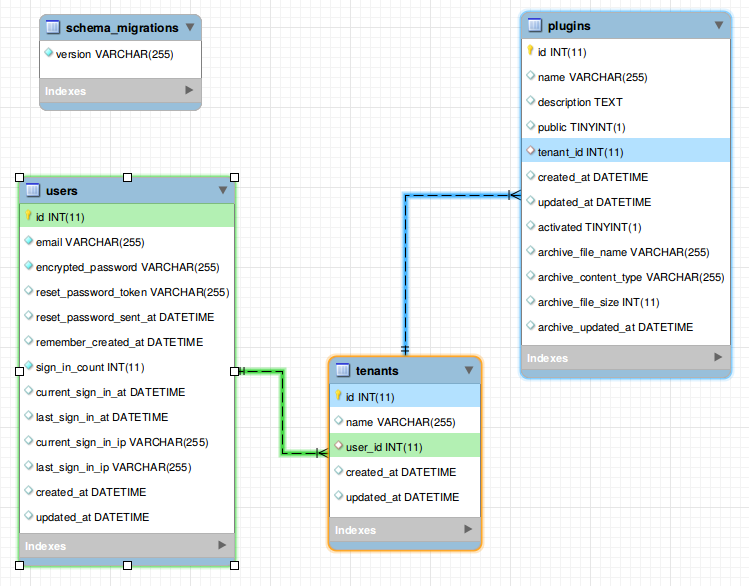
\includegraphics [scale=0.57]{./diagram-db}
  \caption {Диаграма на структурата на базата данни}
\end{figure}

\chapter {Програмна реализация}
\section {Архитектура и структура на системата}
\subsection {Компоненти на системата}
\subsubsection {Docker}
Docker се грижи за разделянето на отделните наематели на системата в изолирани контейнери. Всеки наемател представлява уеб приложение, работещо в контейнер. За да може да бъде достъпено уеб приложението, контейнера трябва да разкрвива към системата мрежовия порт, върху който работи уеб приложението. (Това се налага, защото по подразбиране, мрежовите портове на контейнерите са изолирани от тези на системата.)
\subsubsection {nginx}
nginx служи за да анализирa заявките и да ги пренасочва към правилния наемател (контейнер) или към Videira\footnote{За повече информация за Videira: секция 3.1.1.5}. Ако заявката е към главния домейн (http://domain.xyz), тя бива пренасочвана към Videira. Ако заяквата е към някой поддомейн (http://subdomain.domain.xyz), тя бива пренасочвана към контейнера с име ''subdomain''.\\\\
\begin{figure}[H]
  \centering
  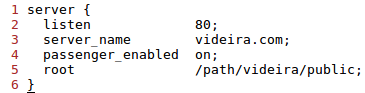
\includegraphics[scale=0.8]{./snippets/nginx_main_server}
  \caption{Примерен сървърен блок от конфигурацията на nginx}
\end{figure}
Нека разгледаме инструкциите в блока, показан на фигура 3.1:
\begin{itemize}
  \item listen: мрежовия порт, на който работи сървъра. (80 е протокола, на който работи Hypertext Transfer Protocol - HTTP).
  \item server\_name: Дава име на виртуалния сървър.
  \item passenger\_enabled: Указва, че заявките към този виртуален сървър трябва да бъдат обслужени от Phussion Passenger (HTTP сървър за уеб приложения, написани на програмния език Ruby).
  \item root: Указва пътя към статичните страници на уеб приложението.
\end{itemize}
\begin{figure}[H]
  \centering
  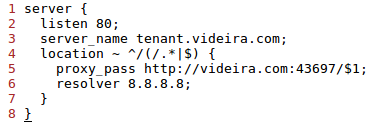
\includegraphics[scale=0.8]{./snippets/nginx_tenant_server}
  \caption{Примерен сървърен блок за наемател от конфигурацията на nginx}
\end{figure}
Във фигура 3.2 виждаме, че са изпуснати инструкциите root и passenger\_enabled, тъй като наемателите се намират в контейнери и достъпваме уеб приложенията в тях, като пренасочваме заявките към мрежовия порт, който контейнера е разкрил. Това пренасочване се извърва от командата location и опциите в нейния блок. След самата ключова дума location е изписан регулярен израз, който съвпада с цялата част от адреса, намираща се след първата ''/'' и присвоява тази част в променливата \$1. Променливата после бива използвана за да се даде пътя от заявката към уеб приложението в контейнера. След самият адрес на сървъра при инструкцията proxy\_pass е добавен мрежовия порт на контейнера. Вътре в този контейнер, работи HTTP сървъра на уеб приложението, който ще обработва заявките, които nginx му пренасочва.
\subsubsection {kamino}
kamino е програма написана на програмния език Go, която използва Docker и nginx за да инсталира нови уеб приложения на сървъра, като те са копия на шаблонното приложение. Шаблонното приложение се записва в специален Docker файл, наречен Docker image (или Docker изображение), който се подава на kamino чрез конфигурационен файл. Конфигурационния файл дава възможност на системния администратор да настрои kamino за да работи по-добре на конкретния сървър. Броя на възможните конфигурационни опции постоянно разсте. На фигура 3.3 е показан един такъв примерен файл, който показва повечето (за момента) опции. \\\\
\begin{figure}[H]
  \centering
  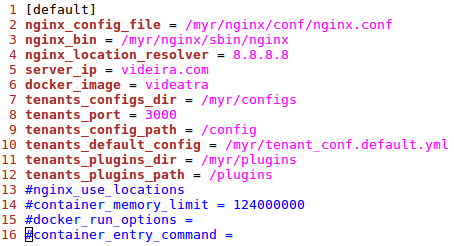
\includegraphics[scale=0.8]{./snippets/config}
  \caption{Конфигурационен файл на kamino}
\end{figure}
kamino е терминална програма, чиято основна функция е командата ``kamino deploy -name=xyz``. При извикването й, програмата първо зарежда конфигурациите от файл и обработва подадените аргументи. При командата deploy това са името на наемателя, който потребителя създава (което задължително трябва да бъде подадено) или мрежовия порт, към който да се пренасочи разкрития от контейнера мрежови порт (ако такава опция не бъде подадена kamino ще намери псевдо произволен свободен мрежови порт). След това ще се извика функцията Deploy, показана на фигура 3.4. Функцията приема като аргументи името на новия наемател и мрежовия порт на операционната система, върху който ще бъде достъпно приложението на новия наемател. Във тялото на Deploy, виждаме функциите dockerRunOptions и dockerRunArguments, които ни дават нужните опции и аргументи за извикването на командата ''docker run'', като ги вземат най-вече от конфигурацията на програмата. kamino приема, че повечето шаблонни приложения ще бъдат разшируеми посредством добавки (plguins) и конфигурация. Поради това, програмата използва функциите makeTenantConfig и makePluginsDir, които създават съответно копие на стандартния конфигурационен за шаблонното приложение файл, който да е личен за наемателя (стандартния конфигурационен файл се определя от конфигурацията на kamino) и лична директория за клиентски добавки. Конфигурационния файл и директорията за добавки по-късно биват вградени (mount-нати) във файловата система на контейнера на наемателя. След това се създава контейнера, чрез Docker и се добавя конфигурация за nginx, в зависимост от това, дали администратора е избрал да инсталира приложенията си, така че да се достъпват на поддомейн или чрез пътя на основния URL (тоест tenant.site.xy или site.xy/tenant). Накрая се презарежда nginx, за да може новата настройка да се отрази. Функцията Deploy връща грешка, ако е възникнала такава (използвана е способността на Go за именовани резултати) или nil, ако всичко е протекло добре.
\begin{figure}[H]
  \centering
  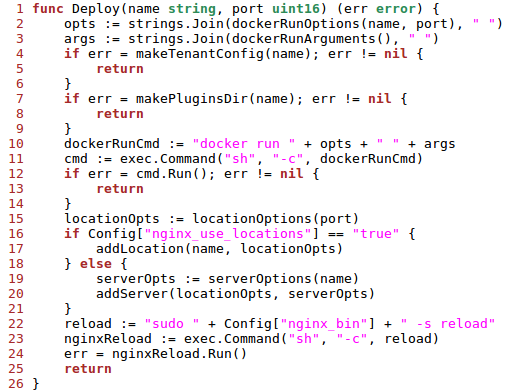
\includegraphics[scale=0.8]{./snippets/kamino_deploy}
  \caption{Функцията, която инсталира нови наематели}
\end{figure}
\subsubsection {Beyond}
beyond е Ruby библиотека (Ruby общността нарича библиотеката gem, но аз ще използвам българския запис ''гем''), която се стреми да предостави цялата функционалност, свързана със създаване и управление на наемателите под формата на Ruby on Rails engine.
\paragraph {Ruby on Rails engine}
Ruby on Rails engine е, най-често, миниатюрно уеб приложение, което предоставя функционалност на своето домакин-приложение. Едно стандартно уеб приложение написано на Rails е всъщност по-частен случай на Rails engine, тъй като класа Rails::Application наследява класа Rails::Engine. Engin-ите се добавят (вграждат) в стандартно Rails приложение и могат да се достъпват на определен път. Обикновено, engine-ите са в отделно именовано пространство, което предотвратява грешки, където едно и също нещо е дефинирано на двете места. Прост пример за Rails engine и неговата употреба може да бъде добавянето на блог engine към дадено уеб приложение. Използвайки engine, можем да добавим функционалността на блога към уеб сайта си, без да променяме програмния код на уеб приложението. Engine-а се добавя много лесно и елегантно към готовото приложение без да рискуваме да го повредим. Друга ползва от този подход е, че един engine може да бъде написан веднъж и преизползван на много места. Това е и причината основната функционалност (като изключим работата, която kamino изпълнява) да бъде изнесена в отделен engine. По този начин всеки администратор, който иска да създаде подобна система за управление на интернет сайтове, може да си инсталира kamino и използвайки beyond да направи единствено приложение, което да съдържа front-end (преден край, интерфейс), който да отговаря на шаблонното приложение.
\paragraph {Начин на работа на beyond}
beyond може да функционира пълноценно, стига да е вградено в някакво приложение. Домакинското приложение не трябва да прави нищо специално за да позволи работата на beyond. beyond съдържа в себе си моделите за User (потребител), Tenant (наемател) и Plugin (добавка). Engine-а използва kamino и Docker за да действия като създаване, пускане и спиране на наематели. Също така beyond може да прилага добавки към наемателското приложение и да управлява неговата конфигурация.
\begin{itemize}
  \item Създаване на наемател се извършва, като се извиква командата ``deploy`` на kamino. За целта, потребителя първо трябва да е влезнал в системата с е-мейл и парола. За всеки новосъздаден наемтаел се създава по един запис/инстанция на модела Tenant.
  \item Спирането и пускането на наемател става чрез ``docker stop`` и ``docker start``.
  \item Конфигурацията на наемател работи по следния начин: първо, при създаването на наемателя, стандартния конфигурационен файл бива копиран във файл, който се намира в указаната в конфигурацията на kamino директория и който носи името на наемателя. След това тази директория бива вградена (mount-ната) в контейнера на наемателя. (тези две операции - копирането и вграждането се извършват от kamino) При достъпване на секцията за промяна на конфигурациите в уеб приложението, конфигурационния файл на съответния наемател бива прочетен и за всяка двойка ключ-стойност се създава поле от съответния тип на стойността. При записване на конфигурациите, файла бива презаписан с новите стойности. На фигура 3.5 е показан примерен конфигурационен файл за шаблонно приложение. Всяка опция съдържа име на опцията, категория на опцията, тип на стойността и стойност.
  \begin{figure}[H]
    \centering
    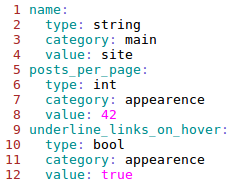
\includegraphics[scale=0.8]{./snippets/tenant_config}
    \caption{Примерен конфигурационен файл за шаблонно приложение}
  \end{figure}
\item Добавките на наемател работят като директорията за добавки на определения наемател се вгради (mount-не) в контейнера му. От приложението се очаква да следи за промяна на файловете в тази директория и да зарежда добавките. Друг начин да се постигне зареждането на добавки е системния администратор да даде команда за презареждането им от тази директория по някакъв начин. Това е възможно понеже beyond дава възможност да изпълнява методи при определени случаи (event-и). Това е напревено чрез проста система за добавки, базирана на гема Plugman. Някои от тези случаи са създаване на наемател, спиране и пускане на наемател и тн. За самото качване на добавките от потребители, beyond използва гема Paperclip, чрез който задълважа добавките да бъдат файлови архиви с разширение tar.gz и да бъдат не по-големи от 10 мегабайта. На фигура 3.6 е показана част от програмния код на модела Plugin, която е свързана с качването на архиви с Paperclip.
  \begin{figure}[H]
    \centering
    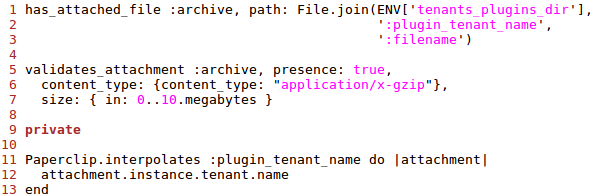
\includegraphics[scale=0.8]{./snippets/plugin_archive}
    \caption{Частта от Plugin модела, която е свързана с качването на архиви с Paperclip}
  \end{figure}
  \item За регистриране, влизане в системата и други стандартни операции за работа с потребители е използван гема Devise, който е сред най-популярните решения за този тип проблеми в областта на Ruby on Rails.
  \item Някои модели в beyond извикват действия от добавките (plugin-и) на beyond при определени случки (event-и). Пример за това е Tenant.deploy. Това е метода, който се извиква, когато клиент на приложението иска да създаде нов наемател. Прост пример за една добавка е показан във фигура 3.7. Добавката записва в файл имената на всички новосъздадени наематели и потребителите, на които те принадлежат.
  \begin{figure}[H]
    \centering
    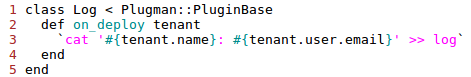
\includegraphics[scale=0.8]{./snippets/beyond_plugin}
    \caption{Примерна добавка за beyond}
  \end{figure}
  \item Дизайна на beyond е сведен до минимум, тъй като целта е engine-а да предоставя само основната функционалност, а изгледите и дизайна, които не са жизненоважни за работата на системата, да бъдат имплементирани от домакинското приложение.
\end{itemize}
\subsubsection {Videira}
Videira е Ruby on Rails приложение, което служи като домакин-приложение за beyond. Videira не имплементира почти никаква функционалност, а се грижи основно за външния вид на уеб сайта и неговия интерфейс. Videira е уеб приложение, което е направено за да създава сайтове за споделяне на видео съдържание. Шаблонното приложение, което то използва е \href{https://github.com/d0ivanov/videatra}{videatra}.\\\\
Цел на Videira е да демонстрира нагледно как един програмист може да използва beyond и да изгради лесно и за много малко време цялостна система, която да може да инсталира и управлява уеб сайтове. За целта програмистът трябва единствено да направи домакин-приложение за beyond, в което да направи свой собствен интерфейс и дизайн.\\\\
Videira използва HAML (алтернатива на HTML, използваща идентация, вместо затварящи тагове) за изгледите си и Twitter Bootstrap за стиловете и динамичното съдържание.\\\\
На фигура 3.8 е показана диаграма описваща структурата на една цялостна система за управление на интернет сайтове. В случая това е Videira.
\begin{figure}[H]
  \centering
  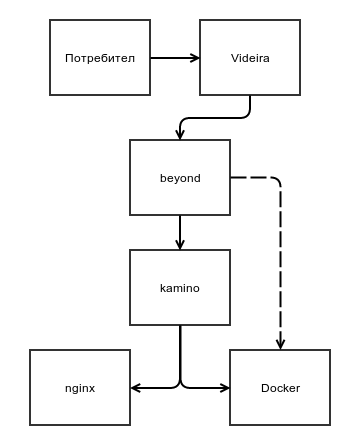
\includegraphics [scale=0.7]{./diagram_all}
  \caption {Диаграма на общата структура на системата}
\end{figure}
На фигура 3.9 е показана началната на страница на Videira, а на 3.10 е демонстрирано таблото за потребителски уебсайтове, където текущия потребител има един уеб сайт, който е в активно състояние.
\floatstyle{boxed}
\restylefloat{figure}
\begin{figure}[H]
  \centering
  
\includegraphics [scale=0.42]{./videira_index}
  \caption {Началната страница на Videira}
\end{figure}
\begin{figure}[H]
  \centering
  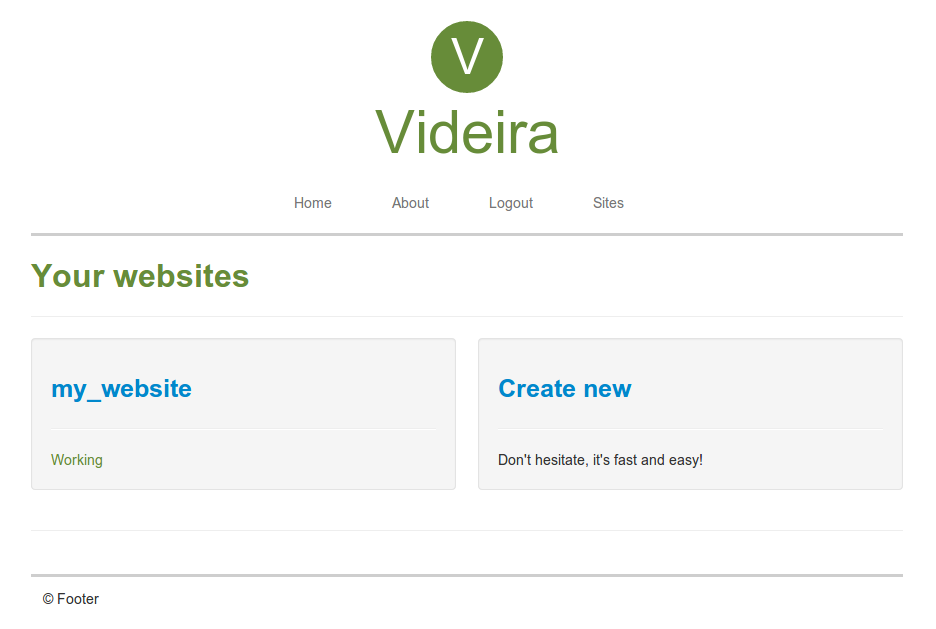
\includegraphics [scale=0.4]{./videira_tenants}
  \caption {Таблото за управление на уеб сайтове във Videira}
\end{figure}
\chapter {Ръководство}
\section {Ръководство за администратора}
\subsection {Изисквания, инсталация и конфигурация на системата}
\subsubsection {Системни изисквания}
Изисква се Linux базирана операционна система, с версия на ядрото (kernel-а) не по-ниска от 3.8, както и следните програми:
\begin{itemize}
  \item Docker  $\ge$ v0.7.2
  \item nginx  $\ge$ v1.4.4
  \item Ruby   $\ge$ v2.0
  \item bundler
\end{itemize}
\subsubsection {Инсталация и конфигурация}
Добра практика е (макар и да не задължително) да се инсталират всичките компоненти на системата в една директория. Например /vid/nginx и /vid/kamino (Docker обикновено бива инсталиран от пакетния мениджър на операционната система, за това го пропускаме). Също така трябва да се създадат две празни директории: за конфигурации и за добавки. Трябва да се създаде и yaml файл (файлов формат използван основно за конфигурации) за настройките по подразбиране на наемателите\footnote{За примерен файл погледни фигура 3.5}. В случай, че шаблонното приложение няма конфигурации, файла може да бъде оставен без съдържание. Няма значение как всички тези директории и файлове биват именовани, тъй като се задават чрез конфигурация на системата. Друго изискване е потребителят (от гледна точна на операционната система), който ще използва системата да бъде добавен към групата ''docker''. Трябва да може да използва също и програмата nginx, без да е нужно да въвежда парола. Потребителят трябва да има права за достъп до конфигурационния файл на nginx, както и до директориите за конфигурации и добавки. Поради тези причини, най-лесно е всичко да бъде инсталирано в една директория, която да принадлежи на потребителя.
\paragraph {Конфигурация на kamino\\}
На фигура 3.3 е показана примерна конфигурация на kamino. Всички опции, описани в нея, които не са коментар са задължителни. Програмата не може да работи без тях (включително и инструкцията ''[default]''). Тук ще бъде обяснено какво представлява всяка от тези опции.
\begin{itemize}
  \item nginx\_config\_file: пътя към конфигурационния файл на nginx.
  \item nginx\_bin:  пътя към изпълнимия файл на nginx.
  \item nginx\_location\_resolver: е IP адреса на DNS сървъра, който превръща имена на сървъри в адреси. 8.8.8.8 е адреса на DNS сървъра на Google. Освен ако не сте сигурни какво правите, най-добре не променяйте тази стойност.
  \item server\_ip: указва IP адреса или домейн името на сървъра ви. Препоръчва се да използвате домейн име, тъй като ако подадете IP адрес, инсталирането на сайтовете на поддомейн няма да работи. Това е защото IP адреса не минава обработка на DNS сървър и не може поддържа така нарчените wildcard записи (записи от вида *.domain.xy, където * съвпада с всяка възможна дума, изградена от валидни символи - букви, цифри, \_, - и тн. ), които са нужни за инсталиране чрез събдомейни.  Ако подадете IP адрес, ще трябва да добавите и опцията ''nginx\_use\_location = true'', която инсталира уеб сайтовете на път от вида domain.xy/sitename. Инсталирането чрез път (втория вариант) е потенциално опасно, понеже може да се получат противоречия с beyond или домакин-приложението на beyond. (ако например домаик-приложението дефинира път /path и инсталирания уеб сайт се казва path - следователно достъпен на /path)
  \item docker\_image: името на Docker ''изображението'', което ще бъде използвано за шаблонно приложение.
  \item tenants\_configs\_dir: пътя към директорията, в която ще се намират всички конфигурации за всички наематели.
  \item tenants\_config\_path: пътя към конфигурационния файл в контейнера. (мястото където конфигурационния файл за дадения наемтаел ще се вгради/mount-не, след като се вземе от tenants\_configs\_dir)
  \item tenants\_port: мрежовия порт, на който работи приложението, което се намира в контейнера. Този порт ще бъде ''открит'' от контейнера и произволен мрежови порт от операционната система ще бъде пренасочен към него. При създаването на нов наемател се избира на произволен принцип свободен мрежови порт, който бива пренасочен към указания от тази опция порт в контейнера.
  \item tenants\_default\_config: конфигурацията по подразбиране, която при създаването на всеки нов наемател ще се копира в директорията за конфигурации (по едно ново копие за всеки наемтаел), а от там ще се вгражда/mount-ва в контейнера за да може приложението в контейнера да я използва.
  \item tenants\_plugins\_dir: същото като tenants\_configs\_dir, но за добавки.
  \item tenants\_plugins\_path: същото като tenants\_config\_path, но за добавки.
  \item Незадължителна: nginx\_use\_locations: при стойност равна на ''true'' инсталира приложенията на път след основния домейн, вместо на поддомейни.
  \item Незадължителна: container\_memory\_limit: лимит на оперативната памет, която контейнерите могат да използват. Мерната единица е байтове.
  \item Незадължителна: docker\_run\_options: допълнителни опции за ''docker run''.
  \item Незадължителна: container\_entry\_command: команда, която да бъде извикана при създаването на нов контейнер.
\end{itemize}
\paragraph {Уеб приложението\\}
За да се даде достъп на потребителите до функционалността на kamino и beyond, трябва да се направи просто Ruby on Rails базирано уеб приложение, което да вгражда в себе си (mount-ва) beyond. Това фронтално (front-end) приложение поема отговорността да предостави потребителски интерфейс и графичен дизайн, които липсват в beyond. В общия случай, nginx се конфигурира така, че това приложение да е достъпно на domain.xy, а от конфигурацията на kamino се прави наемателите да се инсталират на поддомейни на domain.xy (задавайки domain.xy като стойност на server\_ip). По този начин се създава илюзията, че фронталното приложение и всички наематели са един уеб сайт. Фронталното приложение трябва да има файл /configs/application.yml, в който да има следните три реда (замествайки със съответните пътища):
\begin{itemize}
  \item kamino\_bin: /path/to/kamino
  \item tenants\_plugins\_dir: /path/to/plugins\_dir
  \item tenants\_configs\_dir: /path/to/configs\_dir
\end{itemize}
\section {Ръководство за потребителя}
\end{document}
